\subsubsection{QUBO as an Energy Minimization Problem}\label{sec:qubo-as-an-energy-minimization-problem}

A useful way to think about a QUBO problem is not in terms of optimization, but in terms of \textbf{energy}. Instead of saying ``\emph{find the variable assignment that minimizes the objective function}'', we can equivalently say ``\textbf{\emph{find the configuration of variables with the lowest energy}}''. In fact, the objective function:
\begin{equation*}
    y = \mathbf{x}Q\mathbf{x}^T
\end{equation*}
Can be interpreted as an \textbf{energy function} associated with a particular configuration of the binary variables. Every possible assignment of the variables corresponds to a different energy value.

\highspace
\begin{flushleft}
    \textcolor{Green3}{\faIcon{tools} \textbf{Configurations and Energies}}
\end{flushleft}
Consider a simple problem with two \textbf{binary variables}:
\begin{equation*}
    x_{1}, x_{2} \in \{0, 1\}
\end{equation*}
There are \textbf{four possible configurations} of these variables:
\begin{equation*}
    \left(0,0\right), \, \left(0,1\right), \, \left(1,0\right), \, \left(1,1\right)
\end{equation*}
For each configuration, the \textbf{QUBO function produces} a numerical value:
\begin{equation*}
    y(x_{1}, x_{2})
\end{equation*}
This value can be interpreted as the \textbf{energy associated with that configuration}.

\begin{table}[!htp]
    \centering
    \begin{tabular}{@{} c c @{}}
        \toprule
        \textbf{Configuration} & \textbf{Energy} \\
        \midrule
        $(0, 0)$ & $y(0, 0) = E_{1}$ \\
        $(0, 1)$ & $y(0, 1) = E_{2}$ \\
        $(1, 0)$ & $y(1, 0) = E_{3}$ \\
        $(1, 1)$ & $y(1, 1) = E_{4}$ \\
        \bottomrule
    \end{tabular}
\end{table}

\noindent
The optimization problem then becomes the \textbf{search for the configuration with the smallest energy}. In physics, the \hl{state} with the \hl{lowest possible energy} is called the \definition{Ground State}. Thus, solving a QUBO problem is equivalent to finding:
\begin{equation*}
    \mathbf{x}_{\text{opt}} = \argmin_{\mathbf{x}} \mathbf{x} Q \mathbf{x}^T
\end{equation*}
Where $\mathbf{x}_{\text{opt}}$ is the optimal solution, i.e., the configuration corresponding to the ground state of the energy function. \hl{This terminology is extremely important} because later we will \hl{map the QUBO objective function to a quantum Hamiltonian}. At that point, the optimization problem will become simply the problem of finding the ground state of a quantum system. In other words, the \textbf{mathematical problem remains the same}; only the \textbf{interpretation changes}.

\highspace
\begin{flushleft}
    \textcolor{Green3}{\faIcon{book} \textbf{Energy Landscape (useful for visualization)}}
\end{flushleft}
It is often useful to visualize a QUBO problem as an \textbf{energy landscape}. Each possible \textbf{configuration of the variables} corresponds to a \textbf{point in this landscape}, while the \textbf{value} of the \textbf{objective function determines its height}:
\begin{itemize}
    \item[\textcolor{Red2}{\faIcon{times}}] High energy: \textbf{undesirable} solution.
    \item[\textcolor{DarkOrange3}{\faIcon{balance-scale}}] Low energy: \textbf{desirable} solution.
    \item[\textcolor{Green3}{\faIcon{check}}] Minimum energy: \textbf{optimal} solution (ground state).
\end{itemize}
Conceptually, solving the optimization problem is like searching for the deepest valley in the landscape. The global minimum corresponds to the solution of the QUBO problem.

\begin{examplebox}[: QUBO Energy Landscape]
    For example, consider the following QUBO function:
    \begin{equation*}
        E(x_1, x_2) = 1 - x_1 - x_2 + 2x_1 x_2
    \end{equation*}
    This function assigns an energy value to each of the four configurations of the binary variables $x_1$ and $x_2$. We can visualize this energy landscape in a 3D plot, where the $x$ and $y$ axes represent the \textbf{binary variables}, and the $z$ axis represents the \textbf{energy value}. The points corresponding to the four configurations will have different heights based on their energy values, and the \hl{optimal solutions will be the points with the lowest height} (energy).

    \begin{center}
        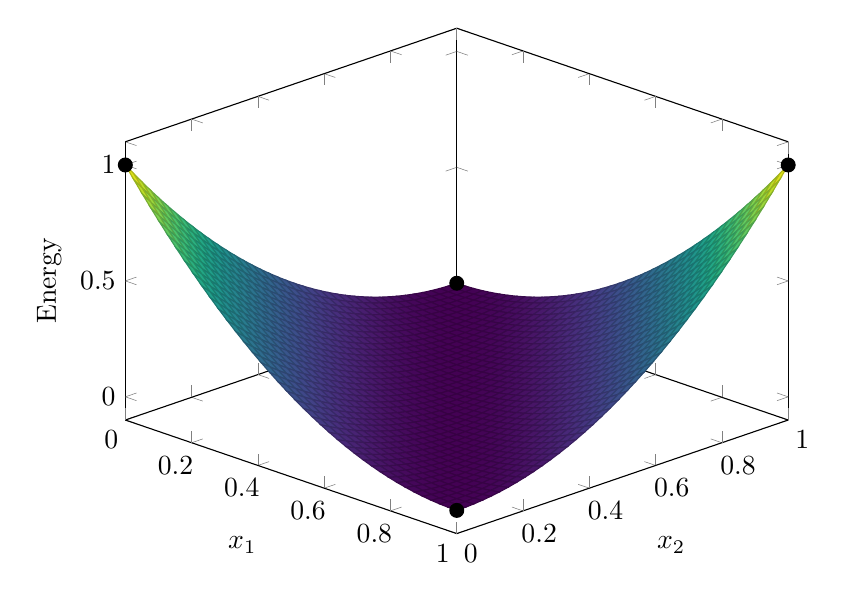
\begin{tikzpicture}
            \begin{axis}[
                view={45}{30},
                xlabel={$x_1$},
                ylabel={$x_2$},
                zlabel={Energy},
                width=10cm,
                height=8cm,
                domain=0:1,
                y domain=0:1,
                samples=40,
                samples y=40,
                colormap/viridis,
            ]
            \addplot3[
                surf,
            ]
            {(x + y - 1)^2};

            \addplot3[
                only marks,
                mark=*,
                mark size=2.5pt,
            ]
            coordinates {
                (0,0,1)
                (0,1,0)
                (1,0,0)
                (1,1,1)
            };
            \end{axis}
        \end{tikzpicture}
    \end{center}
\end{examplebox}

\noindent
In summary, the QUBO formulation can be viewed as an energy minimization problem, where the objective function represents an energy landscape. The goal is to find the configuration of binary variables that corresponds to the lowest energy, which is equivalent to solving the original optimization problem. This perspective is particularly \hl{useful when we later map QUBO problems to quantum Hamiltonians}, as it allows us to leverage concepts from quantum mechanics to find optimal solutions.